% \documentclass[compress]{beamer} % full
\documentclass[handout,compress]{beamer} % no animations

\usepackage{etex} % necessary for pgfplots

\usetheme{AGH}

\graphicspath{{figures/}}
\hypersetup{colorlinks, pdfstartview=FitH, bookmarksopen, pdfpagemode=UseNone, pdfpagemode=UseOutlines, linkcolor=black, citecolor=black, filecolor=black, urlcolor=black, pdfauthor={Piotr Cholda}}

% Not all of the following packages are necessary, but the teacher uses many of them :)
% \usepackage{algorithm}
% \usepackage{algpseudocode}
% \usepackage{amsmath,amsfonts}
% \usepackage{amssymb}
% \usepackage{array,supertabular}
\usepackage{bibentry}
% \usepackage{bm}
\usepackage{booktabs}
% \usepackage{cases}
\usepackage{cite}
\usepackage{color}
\definecolor{gold}{HTML}{E6B800}
\definecolor{lightgreen}{HTML}{99CC00}
\definecolor{blue}{HTML}{4D94DB}
\usepackage{colortbl}
\usepackage{comment}
% \usepackage{dsfont}
\usepackage{enumerate}
\usepackage{exscale,relsize}
\usepackage{floatflt}
\usepackage[OT4]{fontenc}
\usepackage{graphicx}
\usepackage[latin2]{inputenc}
% \usepackage{longtable}
% \usepackage{marvosym}
% \usepackage{multirow}
\usepackage{nicefrac}
\usepackage{paralist}
\usepackage{rotating}
\usepackage[tight,footnotesize]{subfigure}
\usepackage{tabularx}
\usepackage{tabulary}
\usepackage{tikz}
\usetikzlibrary{arrows}
\usetikzlibrary{automata}
\usetikzlibrary{backgrounds}
\usetikzlibrary{calc}
\usetikzlibrary{decorations.pathreplacing}
\usetikzlibrary{decorations.pathmorphing}
\usetikzlibrary{fit}
\usetikzlibrary{matrix}
\usetikzlibrary{mindmap}
\usetikzlibrary{patterns}
\usetikzlibrary{petri}
\usetikzlibrary{positioning}
\usetikzlibrary{plothandlers}
\usetikzlibrary{plotmarks}
\usetikzlibrary{shadings}
\usetikzlibrary{shadows}
\usetikzlibrary{shapes}
\usetikzlibrary{shapes.gates.logic.US}
\usetikzlibrary{topaths}
\usetikzlibrary{trees}
\usepackage{pgfplots} % needs \usepackage{etex} just after \documentclass
\pgfplotsset{tick scale binop=\times}

\usepackage{trfsigns}
\usepackage{url}
\usepackage{wasysym}
\usepackage{wrapfig}

\setbeamertemplate{footline}[text line]{
    \leavevmode
    \hbox{
        \begin{beamercolorbox}[wd=\paperwidth,ht=0.01ex,dp=0ex,leftskip=0.25cm,rightskip=0cm plus1fil]{title in head/foot}
            \usebeamerfont{title in head/foot}\logosinfootline
        \end{beamercolorbox}
    }
}

\setbeamertemplate{frametitle continuation}[from second][\insertcontinuationtext]

\setbeamercovered{dynamic}
\definecolor{lightgreen}{RGB}{218,238,225}
\setbeamercolor{rafi}{fg=lightgreen,bg=}

\newenvironment{changemargin}[2]{%
    \begin{list}{}{%
        \setlength{\topsep}{0pt}%
        \setlength{\leftmargin}{#1}%
        \setlength{\rightmargin}{#2}%
        \setlength{\listparindent}{\parindent}%
        \setlength{\itemindent}{\parindent}%
        \setlength{\parsep}{\parskip}%
    }%
    \item[]}
{\end{list}}

% \bstctlcite
\makeatletter
    \def\bstctlcite#1{\@bsphack
    \@for\@citeb:=#1\do{%
    \edef\@citeb{\expandafter\@firstofone\@citeb}%
    \if@filesw\immediate\write\@auxout{\string\citation{\@citeb}}\fi}%
    \@esphack}
\makeatother

\newtheorem{remark}{Remark}[theorem]

\abovedisplayshortskip=0pt

\DeclareMathOperator*{\argmin}{arg\,min}

\DeclareMathOperator*{\erf}{erf}

\DeclareMathOperator*{\rank}{rank}

\DeclareMathOperator*{\Dom}{Dom}

\DeclareMathOperator*{\opt}{opt}

\DeclareMathOperator*{\conv}{conv}

\DeclareMathOperator*{\diff}{\!\text{d}}

\DeclareMathOperator*{\mean}{\text{E}}

\DeclareMathOperator*{\logistic}{\text{logistic}}

\newcommand{\eqdef}{%
      \ensuremath{%
          \stackrel{\text{def}}{=}%
      }%
  }

%%%%%%%%%%%%%%%%%%%%%%%%%%%%%%%%%%%%%%%%%%%%%%%%%%%%%%%%%%%%%%%%%%%%%%%%%%%%%%%%%%%%%%%%%%%%%%%%%%%
%%%%%%%%%%%%%%%%%%%%%%%%%%%%%%%%%%%%%%%%%%%%%%%%%%%%%%%%%%%%%%%%%%%%%%%%%%%%%%%%%%%%%%%%%%%%%%%%%%%
%%%%%%%%%%%%%%%%%%%%%%%%%%%%%%%%%%%%%%%%%%%%%%%%%%%%%%%%%%%%%%%%%%%%%%%%%%%%%%%%%%%%%%%%%%%%%%%%%%%
%%%%%%%%%%%%%%%%%%%%%%%%%%%%%%%%%%%%%%%%%%%%%%%%%%%%%%%%%%%%%%%%%%%%%%%%%%%%%%%%%%%%%%%%%%%%%%%%%%%
%%%%%%%%%%%%%%%%%%%%%%%%%%%%%%%%%%%%%%%%%%%%%%%%%%%%%%%%%%%%%%%%%%%%%%%%%%%%%%%%%%%%%%%%%%%%%%%%%%%
\title%<<<<<<<<<<<<<<<<<<<<<<<<<<<<<<<<<<<<<<<<<<<<<<<<<<<<<<<<<<<<<<<<<
{Seminar in \emph{Artificial Intelligence}}
\subtitle{}
\author[]{Marcin Zajac, Dominik Koza, Lukasz Gorczyca}
\institute[KT AGH]{Department of Telecommunications}%
\date{01.04.2019} % Change, please!
%%%%%%%%%%%%%%%%%%%%%%%%%%%%%%%%%%%%%%%%%%%%%%%%%%%%%%%%%%%%%%%%%%%%%%%%%%%%%%%%%%%%%%%%%%%%%%%%%%%
%%%%%%%%%%%%%%%%%%%%%%%%%%%%%%%%%%%%%%%%%%%%%%%%%%%%%%%%%%%%%%%%%%%%%%%%%%%%%%%%%%%%%%%%%%%%%%%%%%%
%%%%%%%%%%%%%%%%%%%%%%%%%%%%%%%%%%%%%%%%%%%%%%%%%%%%%%%%%%%%%%%%%%%%%%%%%%%%%%%%%%%%%%%%%%%%%%%%%%%
%%%%%%%%%%%%%%%%%%%%%%%%%%%%%%%%%%%%%%%%%%%%%%%%%%%%%%%%%%%%%%%%%%%%%%%%%%%%%%%%%%%%%%%%%%%%%%%%%%%
%%%%%%%%%%%%%%%%%%%%%%%%%%%%%%%%%%%%%%%%%%%%%%%%%%%%%%%%%%%%%%%%%%%%%%%%%%%%%%%%%%%%%%%%%%%%%%%%%%%

\begin{document}

\begin{frame}
    \titlepage
    \nobibliography* % Necessary if literature is given
\end{frame}

\setbeamertemplate{background}{
\includegraphics[width=\paperwidth,height=\paperheight]{./files/tlo}}

\renewcommand{\logosinfootline}{\raisebox{0.12cm}{\begin{beamercolorbox}{rafi}{Seminar \quad Overview regression methods \hfill \insertframenumber/\inserttotalframenumber}\end{beamercolorbox}}}
%%%%%%%%%%%%%%%%%%%%%%%%%%%%%%%%%%%%%%%%%%%%%%%%%%%%%%%%%%%%%%%%%%%%%%%%%%%%%%%%%%%%%%%%%%%	   
%%%%%%%%%%%%%%%%%%%%%%%%%%%%%%%%%%%%%%%%%%%%%%%%%%%%%%%%%%%%%%%%%%%%%%%%%%%%%%%%%%%%%%%%%%%	   
\begin{frame}[allowframebreaks]
	\frametitle{1. Agenda}
    \begin{itemize}
    \item 1. Intro, presentation plan.
    \item 2. What is regression?
    \item 3. What regression is used for?
    \item 4. Types of regression.
    \item 5. Simple Linear regression.
    \item 6. Multiple dimension extension.
    \item 7. Ordinary least squares.
    \item 8. Gradient descent in linear regression.
    \item 9. Regularization - Ridge and Lasso
    \item 10. Logistic regression.
    \item 11. Polynominal regression.
    \item 12. QA
	\end{itemize}
\end{frame}
%%%%%%%%%%%%%%%%%%%%%%%%%%%%%%%%%%%%%%%%%%%%%%%%%%%%%%%%%%%%%%%%%%%%%%%%%%%%%%%%%%%%%%%%%%%	   
%%%%%%%%%%%%%%%%%%%%%%%%%%%%%%%%%%%%%%%%%%%%%%%%%%%%%%%%%%%%%%%%%%%%%%%%%%%%%%%%%%%%%%%%%%%	   
\begin{frame}
	\frametitle{2/3. What is regression? What is used for?}
	\begin{itemize}
	\item looks for the relationship between two or more variables.
	\item used in: forecasting, MS Excel :D, Machine Learning...
\end{itemize}		
\end{frame}
%%%%%%%%%%%%%%%%%%%%%%%%%%%%%%%%%%%%%%%%%%%%%%%%%%%%%%%%%%%%%%%%%%%%%%%%%%%%%%%%%%%%%%%%%%%
%%%%%%%%%%%%%%%%%%%%%%%%%%%%%%%%%%%%%%%%%%%%%%%%%%%%%%%%%%%%%%%%%%%%%%%%%%%%%%%%%%%%%%%%%%%
\begin{frame}
	\frametitle{4. Types of regression}
	\begin{itemize}
	\item linear regression
	\item logistic regression
	\item polynominal regression
	\item stepwise regression
	\item ridge regression
	\item lasso regression
	\item elasticNet regression
\end{itemize}		
\end{frame}

%%%%%%%%%%%%%%%%%%%%%%%%%%%%%%%%%%%%%%%%%%%%%%%%%%%%%%%%%%%%%%%%%%%%%%%%%%%%%%%%%%%%%%%%%%%
%%%%%%%%%%%%%%%%%%%%%%%%%%%%%%%%%%%%%%%%%%%%%%%%%%%%%%%%%%%%%%%%%%%%%%%%%%%%%%%%%%%%%%%%%%%

\begin{frame}[allowframebreaks]
    \frametitle{5. Linear regression}	
    	\begin{itemize}
	\item First known research in this area --- method of least squares published by Legendre in 1805 and by Gauss in 1809.
	\item
	The representation is a linear equation that combines a specific set of input values x the solution to which is the predicted output for that set of input values y. As such, both the 		input values x and the output value are numeric.
	\end{itemize}
	\end{frame}
%%%%%%%%%%%%%%%%%%%%%%%%%%%%%%%%%%%%%%%%%%%%%%%%%%%%%%%%%%%%%%%%%%%%%%%%%%%%%%%%%%%%%%%%%%%	  
%%%%%%%%%%%%%%%%%%%%%%%%%%%%%%%%%%%%%%%%%%%%%%%%%%%%%%%%%%%%%%%%%%%%%%%%%%%%%%%%%%%%%%%%%%%	    	
	\frame{
	    \frametitle{5. Simple Linear Regression}
	    	\begin{itemize}
	    		\item Simple linear regression is a linear regression model with a single independent variable.
			\item Model for single dimension: \pause
			\begin{equation}
				y_{i} = \beta_{0} + \beta_{1}x_{i}+\epsilon_{i}
			\end{equation}
			\item Naming: \pause
			\begin{itemize}
				\item The unknown parameters --- $\beta$
				\item The independent variables --- $X$ or $x$ \pause
				\item The dependent variable ---  $Y$ or $y$   \pause
				\item Introduced error ---  $\epsilon$ \pause
			\end{itemize}
		\end{itemize}
	}
%%%%%%%%%%%%%%%%%%%%%%%%%%%%%%%%%%%%%%%%%%%%%%%%%%%%%%%%%%%%%%%%%%%%%%%%%%%%%%%%%%%%%%%%%%%	   %%%%%%%%%%%%%%%%%%%%%%%%%%%%%%%%%%%%%%%%%%%%%%%%%%%%%%%%%%%%%%%%%%%%%%%%%%%%%%%%%%%%%%%%%%%	   	
	\frame{
	\begin{itemize}
	\frametitle{6. Multiple dimension extension}
	\item When there is a single input variable x, the method is referred to as simple linear regression. When there are multiple input variables, literature from statistics often refers to the method as multiple linear regression.
	\item Model for n dimension:
	\begin{equation}
		y_{i} = \beta_{0} + \beta_{1}x_{i,1}+ \beta_{2}x_{i,2} + ...+ \beta_{n}x_{i,n} + \epsilon_{i}
	\end{equation}
	\item To matrix representation:
	\begin{equation}
		y_{i} = x_{i}^{T} + \epsilon_{i}
	\end{equation}
	\begin{equation}
		Y = X\beta+ \epsilon
	\end{equation}
   	\end{itemize}
	}
%%%%%%%%%%%%%%%%%%%%%%%%%%%%%%%%%%%%%%%%%%%%%%%%%%%%%%%%%%%%%%%%%%%%%%%%%%%%%%%%%%%%%%%%%%%
%%%%%%%%%%%%%%%%%%%%%%%%%%%%%%%%%%%%%%%%%%%%%%%%%%%%%%%%%%%%%%%%%%%%%%%%%%%%%%%%%%%%%%%%%%%	    
	\frame[allowframebreaks]{
	    \frametitle{7. Ordinary least squares}
	    \center Method for estimating the unknown parameters in a linear regression model:
	    	\begin{equation}
			\hat{\beta} = argmin_{\beta} S(\beta)
		\end{equation}
		\begin{equation}
			S(\beta) = \sum_{i=1}^{n} \mid y_i-\sum_{j=1}^{p}X_{ij}\beta_{j} \mid ^{2}
		\end{equation}
		\begin{figure}[h]
		\centering 
		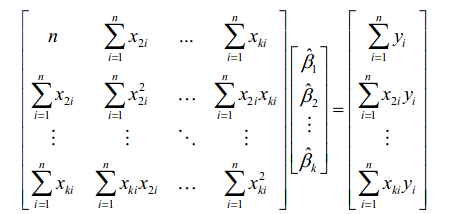
\includegraphics[scale=0.3]{images/matrix1.png}
		\end{figure}
		\center Which leads to:
		\begin{figure}[h]
		\centering 
		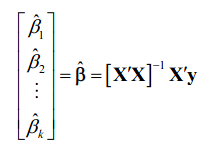
\includegraphics[scale=0.5]{images/matrix2.png}
		\end{figure}
	   }
%%%%%%%%%%%%%%%%%%%%%%%%%%%%%%%%%%%%%%%%%%%%%%%%%%%%%%%%%%%%%%%%%%%%%%%%%%%%%%%%%%%%%%%%%%%
%%%%%%%%%%%%%%%%%%%%%%%%%%%%%%%%%%%%%%%%%%%%%%%%%%%%%%%%%%%%%%%%%%%%%%%%%%%%%%%%%%%%%%%%%%%	   	   
	\frame[allowframebreaks]{
	    \frametitle{8. Gradient descent in linear regression}
	    \vspace{-0.4cm}
	    Gradient descent is a first-order iterative optimization algorithm for finding the minimum of a function.
	    \\Denote E as squared mean error in example for linear regression:
	    \begin{equation}
	    E=1/n \times \sum_{i=0}^{n}(y_{i}-\beta_{1}\times x_{i}+\beta_{0})
	    \end{equation}
	    Let us assume that:
	    \begin{equation}
	    a=\beta_{1}
	    \end{equation}
	    \begin{equation}
	    b=\beta_{0}
	    \end{equation}
	    \begin{equation}
	    D_{a}=\frac{\mathrm d}{\mathrm d a} \left( E \right)
	    \end{equation}
	    \begin{equation}
	    D_{b}=\frac{\mathrm d}{\mathrm d b} \left( E \right)
	    \end{equation}
	    Now find that a and b where function E will reach minimum or be small enough. Take some $L$ as learning rate and iterative find values of a and b from equations:
	    \begin{equation}
	    a=a-L\times D_{a}
	    \end{equation}
	    \begin{equation}
	    b=b-L\times D_{b}
	    \end{equation}
	    		\begin{figure}[h]
		\centering 
		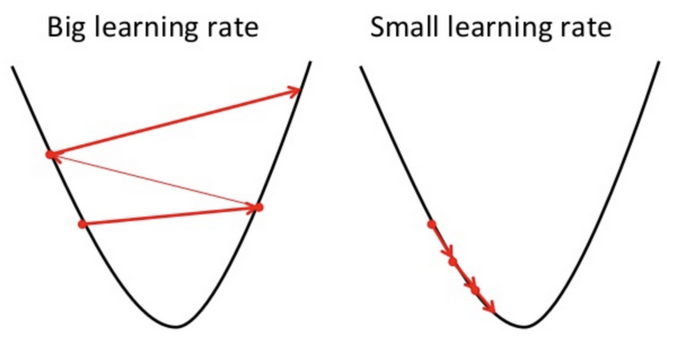
\includegraphics[scale=0.45]{images/smallBigLR.png}
		\end{figure}
		Training rate $L$ has to be small enough to avoid skipping minimum.
	   }
%%%%%%%%%%%%%%%%%%%%%%%%%%%%%%%%%%%%%%%%%%%%%%%%%%%%%%%%%%%%%%%%%%%%%%%%%%%%%%%%%%%%%%%%%%%
%%%%%%%%%%%%%%%%%%%%%%%%%%%%%%%%%%%%%%%%%%%%%%%%%%%%%%%%%%%%%%%%%%%%%%%%%%%%%%%%%%%%%%%%%%%	   	   	 
	 \frame{
	    \frametitle{9. Regularization}
	    Regularization methods provide a means to control our regression coefficients, which can reduce the variance and decrease our of sample error.
	    \\Two popular examples of regularization procedures for linear regression are:
	\begin{itemize}
    \item Lasso Regression --- called L1 regularization.
    \item Ridge Regression --- called L2 regularization.
\end{itemize}
These methods are effective to use when there is collinearity in your input values and ordinary least squares would overfit the training data.
	   }
	   	
	   	 \frame[allowframebreaks]{
	   	 \frametitle{9. Regularization}
	   	 \framesubtitle{Ridge Regression}
	   	 Ridge should be used if we want to remain all parameters.
	   	\begin{equation}
	    E=1/n \times \sum_{i=0}^{n}(y_{i}-\beta_{1}\times x_{i}+\beta_{0})
	    \end{equation}
	    Adding Ridge penalty:
	   	\begin{equation}
	    \min (E+\lambda \sum_{j=1}^{p}\beta_{j}^{2})
	    \end{equation}	
	   	\begin{figure}[h]
		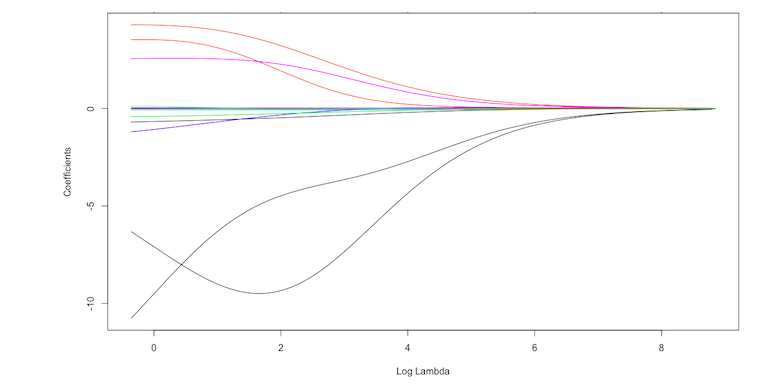
\includegraphics[scale=0.3]{images/ridge.png}
		\end{figure}
		We see that Ridge remain all variables and with incrementing $\lambda$ all are forced to 0.
		To find $\lambda$ we can also perform CV.
		}
		\frame[allowframebreaks]{
	   	 \frametitle{9. Regularization}
	   	 \framesubtitle{Ridge Regression - Example}
		\begin{figure}[h]
		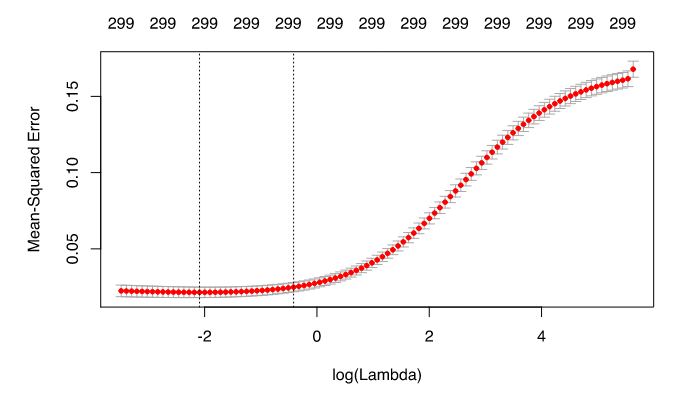
\includegraphics[scale=0.3]{images/cvRidge.png}
		\end{figure}
		In this case Ridge is not providing improvements. What about Lasso?
	   	 }
	   	 
	   	 \frame[allowframebreaks]{
	   	 \frametitle{9. Regularization}
	    \framesubtitle{Lasso Regression}
	    Lasso allows to get rid of some parameters. 
	   	\begin{equation}
	    E=1/n \times \sum_{i=0}^{n}(y_{i}-\beta_{1}\times x_{i}+\beta_{0})
	    \end{equation}
	    Adding Lasso penalty:
	   	\begin{equation}
	    minimize(E+\lambda \sum_{j=1}^{p}|\beta_{j}|)
	    \end{equation}	
	   	\begin{figure}[h]
		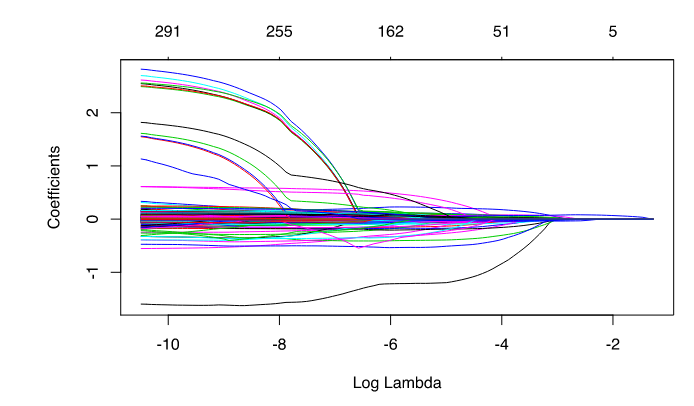
\includegraphics[scale=0.3]{images/lasso1.png}
		\end{figure}
	    How to find $\lambda$? We can perform cross-validation.
	    Example: 
	   	\begin{figure}[h]
		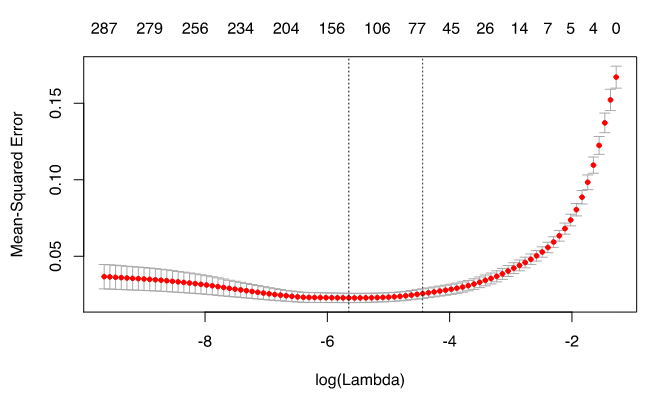
\includegraphics[scale=0.3]{images/lassoCV.png}
		\end{figure}
		There is improvement but some coefficients are equals to 0 which indicades that some parameters will not be taken into consideration.
	     }
%%%%%%%%%%%%%%%%%%%%%%%%%%%%%%%%%%%%%%%%%%%%%%%%%%%%%%%%%%%%%%%%%%%%%%%%%%%%%%%%%%%%%%%%%%%	   %%%%%%%%%%%%%%%%%%%%%%%%%%%%%%%%%%%%%%%%%%%%%%%%%%%%%%%%%%%%%%%%%%%%%%%%%%%%%%%%%%%%%%%%%%%	   

%%%%%%%%%%%%%%%%%%%%%%%%%%%%%%%%%%%%%%%%%%%%%%%%%%%%%%%%%%%%%%%%%%%%%%%%%%%%%%%%%%%%%%%%%%%
%%%%%%%%%%%%%%%%%%%%%%%%%%%%%%%%%%%%%%%%%%%%%%%%%%%%%%%%%%%%%%%%%%%%%%%%%%%%%%%%%%%%%%%%%%%	   	   	 
\begin{frame}[allowframebreaks]
\frametitle{10. Logistic regression}
\begin{itemize}
	\item 
	Logistic regression was developed by statistician David Cox in 1958 
	\item 
	Logistic Regression is one of the basic and the most popular algorithm to solve a classification problem.
	\item 
	The main idea of logistic regression is to find a relationship between features and probability of particular outcome.
\end{itemize}
\end{frame}

\begin{frame}[allowframebreaks]
\frametitle{10. Logistic regression}
\begin{itemize}
	\item 
	In logistic regression, the dependent variable is binary or dichotomous, i.e. it only contains data coded as 1 (TRUE, success, etc.) or 0 (FALSE, failure, etc.).
	\item
	Linear regression predicts values outside the acceptable range (e.g. predicting probabilities
	outside the range 0 to 1).
	
\end{itemize}
\end{frame}

\begin{frame}[allowframebreaks]
\frametitle{10. Logistic regression}
Function graph:
\begin{itemize}
	\item 
	For the begining arguments values are nearly 0 or 1.
	\item
	After reaching critical value we see dynamically increase/decrease of function  value.
	\item
	For the final arguments values are nearly 1 or 0 (opposite to the begining).
\end{itemize}
		\begin{figure}[h]
		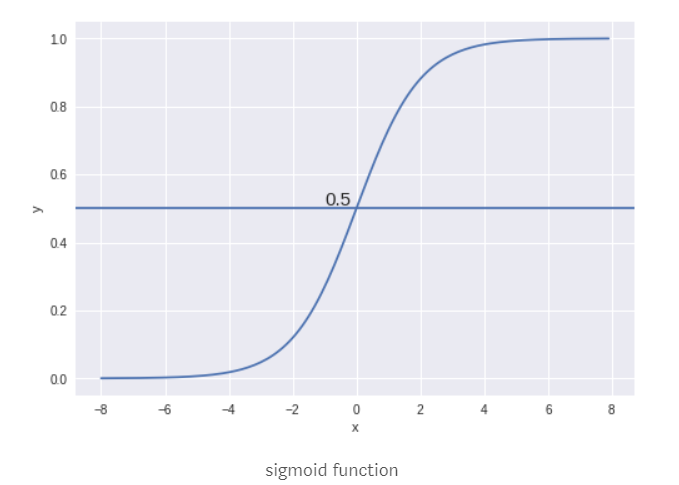
\includegraphics[scale=0.3]{images/lukasz1.png}
		\end{figure}

\end{frame}

\begin{frame}[allowframebreaks]
\frametitle{10. Logistic regression}
\begin{itemize}
	\item
	The biggest difference between linear and logistic regrresion is how the line is fit to the data.
	\item 
	Logistic regression uses maximum likelihood estimation (MLE) to get the model coefficients.
	
\end{itemize}
		\begin{figure}[h]
		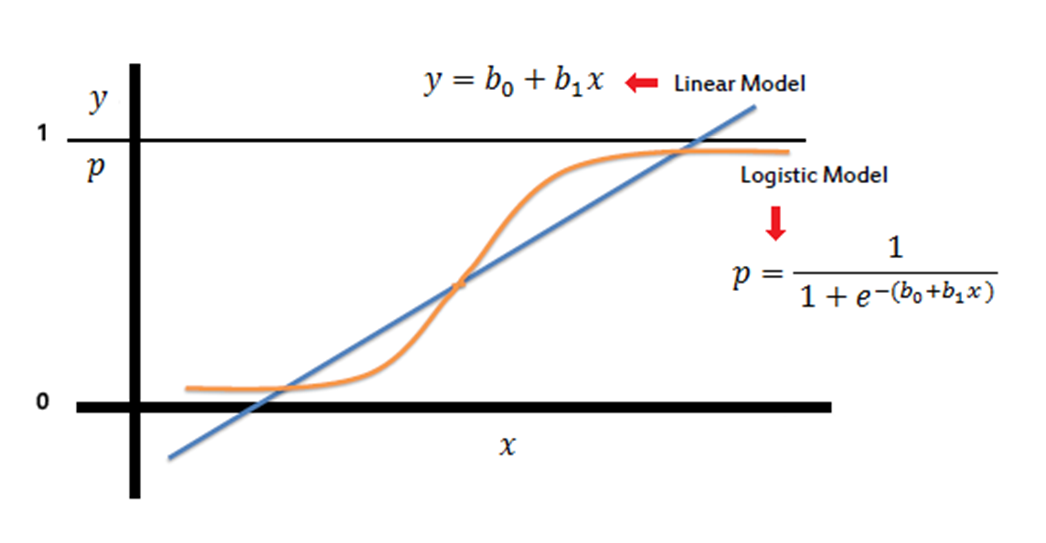
\includegraphics[scale=0.3]{images/lukasz2.png}
		\end{figure}
\end{frame}

\begin{frame}[allowframebreaks]
\frametitle{10. Logistic regression}
Why should we use logistic regression instead of linear?
\begin{itemize}
\item
Let \textbf{x} be some feature and \textbf{y} be the output which can be either 0 or 1. 
\item
The probability that the output is 1 can be represented as:
\begin{equation}
P = (y=1 | x)
\end{equation}
\item
Using linear regression we will get:  
\begin{equation}
p(X) = \beta_{0} + \beta_{1}X
\end{equation}
\item
Logistic regression is expressed by logit function, therefore:
\end{itemize}
\begin{equation}
p(X) = {e^{\beta_{0} + \beta_{1}X}}/{1 + e^{\beta_{0} + \beta_{1}X}}
\end{equation}
\end{frame}

\begin{frame}[allowframebreaks]
\frametitle{10. Logistic regression}
Different types of logistic regression:
\begin{itemize}
	\item
	1. Binary: The categorical response has only two 2 possible outcomes (e.g.: Spam or Not).
	\item
	2. Multinomial: Three or more categories without ordering. (e.g.: Predicting which food is preferred more (Veg, Non-Veg, Vegan)).
	\item
	3. Ordinal: Three or more categories with ordering. (e.g.: Movie rating from 1 to 5).
\end{itemize}
\end{frame}
\begin{frame}[allowframebreaks]
\frametitle{10. Logistic regression}
\framesubtitle{Summing up}
\begin{itemize}
	\item
	Logistic regression's ability to provide probabilities and classify new samples using continuous and discrete measurements makes it a popular machine learning method.
\end{itemize}
\end{frame}
%%%%%%%%%%%%%%%%%%%%%%%%%%%%%%%%%%%%%%%%%%%%%%%%%%%%%%%%%%%%%%%%%%%%%%%%%%%%%%%%%%%%%%%%%%%	   %%%%%%%%%%%%%%%%%%%%%%%%%%%%%%%%%%%%%%%%%%%%%%%%%%%%%%%%%%%%%%%%%%%%%%%%%%%%%%%%%%%%%%%%%%%
	 
	\frame{
	 	\frametitle{11. Polynominal Regression}
		\begin{itemize}
		\item Occurs when regression equation has independent variable in power higher than 1.
		\item General equation:
			\begin{equation}
				y = \beta_{0} + \beta_{1}\times x_{i} + \beta_{2}\times x_{i}^2 + \beta_{3}\times x_{i}^3 + ... + \beta_{m}\times x_{i}^m + E, i=1,2,3...
			\end{equation}
		\item Example (variable in 2 power):
			\begin{equation}
				y = a + b\times x^2			
			\end{equation}
		\item The best fit is rather curve not a straight line.
	 	\end{itemize}
	   }
%%%%%%%%%%%%%%%%%%%%%%%%%%%%%%%%%%%%%%%%%%%%%%%%%%%%%%%%%%%%%%%%%%%%%%%%%%%%%%%%%%%%%%%%%%%	   
%%%%%%%%%%%%%%%%%%%%%%%%%%%%%%%%%%%%%%%%%%%%%%%%%%%%%%%%%%%%%%%%%%%%%%%%%%%%%%%%%%%%%%%%%%%	   
	 \frame{
	    \frametitle{11. Polynominal Regression}
	    \begin{itemize}
	    \item Polynominal with higher degree can give us lower error rate.
	    \item If degree will be too high then overfitting will occur.
	    \item Curve sholud fit the nature of the problem (trend) not every single sample.
	    \end{itemize}
	   }
%%%%%%%%%%%%%%%%%%%%%%%%%%%%%%%%%%%%%%%%%%%%%%%%%%%%%%%%%%%%%%%%%%%%%%%%%%%%%%%%%%%%%%%%%%%	   
%%%%%%%%%%%%%%%%%%%%%%%%%%%%%%%%%%%%%%%%%%%%%%%%%%%%%%%%%%%%%%%%%%%%%%%%%%%%%%%%%%%%%%%%%%%	   
	 \frame{
	    \frametitle{11. Polynominal Regression}	    
	    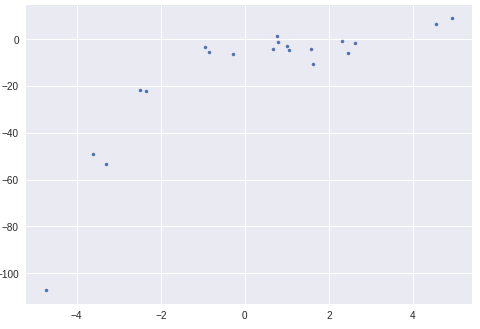
\includegraphics[scale=0.3]{images/sample_data.png}
	    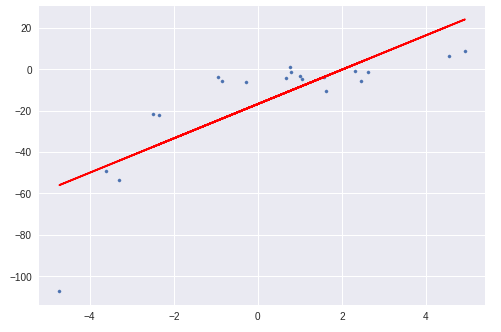
\includegraphics[scale=0.3]{images/linear_regression.png}
	   }
	 \frame{
		\frametitle{11. Polynominal Regression}
		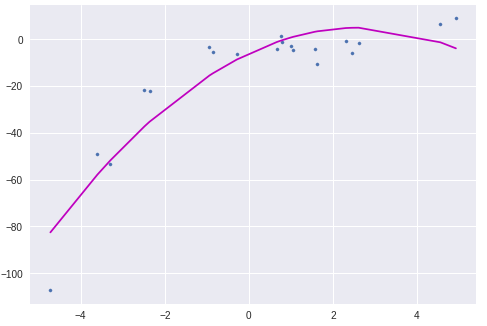
\includegraphics[scale=0.3]{images/2_degree.png}
	    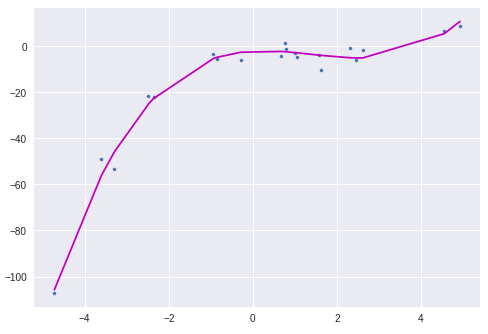
\includegraphics[scale=0.3]{images/3_degree.png}
	 }
	 \frame{
		\frametitle{11. Polynominal Regression}	 
		\begin{center}
		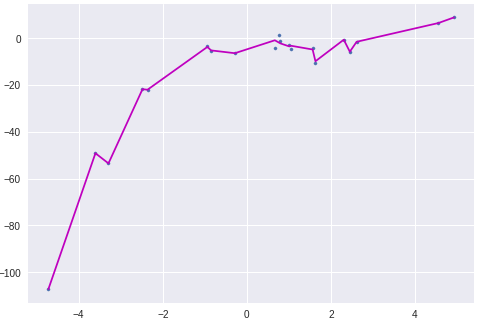
\includegraphics[scale=0.3]{images/20_degree.png}	 
		\end{center}				
		
	 }


%%%%%%%%%%%%%%%%%%%%%%%%%%%%%%%%%%%%%%%%%%%%%%%%%%%%%%%%%%%%%%%%%%%%%%%%%%%%%%%%%%%%%%%%%%%%%
%%%%%%%%%%%%%%%%%%%%%%%%%%%%%%%%%%%%%%%%%%%%%%%%%%%%%%%%%%%%%%%%%%%%%%%%%%%%%%%%%%%%%%%%%%%%%
\begin{frame}
	
	\begin{center}
		\Huge \textbf{Thank you for your attention!}
	\end{center}

\end{frame}
%%%%%%%%%%%%%%%%%%%%%%%%%%%%%%%%%%%%%%%%%%%%%%%%%%%%%%%%%%%%%%%%%%%%%%%%%%%%%%%%%%%%%%%%%%%%%
%%%%%%%%%%%%%%%%%%%%%%%%%%%%%%%%%%%%%%%%%%%%%%%%%%%%%%%%%%%%%%%%%%%%%%%%%%%%%%%%%%%%%%%%%%%%%
\begin{frame}
	
	\begin{center}
		\Huge \textbf{Q \& A}
	\end{center}

\end{frame}
%%%%%%%%%%%%%%%%%%%%%%%%%%%%%%%%%%%%%%%%%%%%%%%%%%%%%%%%%%%%%%%%%%%%%%%%%%%%%%%%%%%%%%%%%%%%%%%%%%%

%%%%%%%%%%%%%%%%%%%%%%%%%%%%%%%%%%%%%%%%%%%%%%%%%%%%%%%%%%%%%%%%%%%%%%%%%%%%%%%%%%%%%%%%%%%%%%%%%%%

\bibliographystyle{plain}
\nobibliography{bibliographyfile} % your bibliography file

\end{document}